%# -*- coding: utf-8-unix -*-
\chapter{双体船的窄V字形尾迹}
\label{chap:catamaran}

\section{引言}
本章将第\ref{chap:monohull}章对单体船窄V字形尾迹的数值研究推广到双体船。
因此本章考虑在无限深广的静水中以航速$V$直线航行的双体船的窄V字形尾迹。
双体船由长$L$、型宽$B$、吃水$D$的两个完全相同的片体组成,片体间距为$S$,
如图\ref{fig:defsketch}所示。无因次化的片体间距$s$定义为
\begin{equation}
  s\equiv S/L
  \label{eq:sdef}
\end{equation}
基于片体间距$S$和船长$L$的Froude数$F_s$和$F$分别是
\begin{subequations}\label{eq:FFsdef}
  \begin{eqnarray}
    &&F_s\equiv V/\sqrt{gS}\equiv F/\sqrt{s}\label{eq:FFsdef-a}\\
    &&F\equiv V/\sqrt{gL}\equiv F_s\sqrt{s}\label{eq:FFsdef-b}
  \end{eqnarray}
\end{subequations}
这里$g$是重力加速度。双体船产生的波浪从固结于船体随船体一起运动的Galilean坐标系
观测。$Z$轴竖直向上,并将未扰动的自由面取为$Z=0$。$X$轴沿着船的航向,位于两片体
之间。片体关于平面$Y=\pm S/2$对称。定义无因次坐标
\begin{equation}
  (x,y,z)\equiv(X,Y,Z)/L
  \label{eq:xyz}
\end{equation}
%
\begin{figure}[htp]
  \centering
  \captionstyle{\centering}
  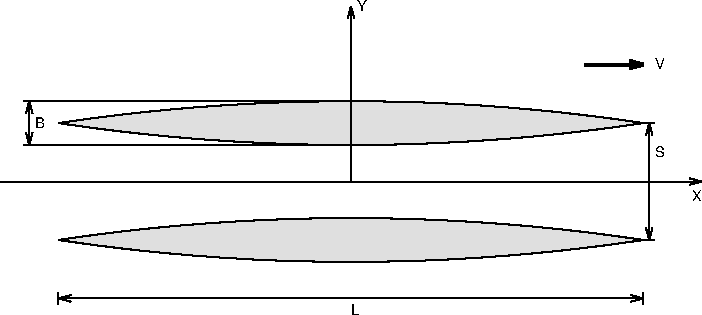
\includegraphics[width=0.8\textwidth]{chap6/def_sket.pdf}
  \bicaption[fig:defsketch]{双体船俯视图}
  {一艘由长$L$、型宽$B$、吃水$D$的两个完全相同的间距为$S$
  的片体组成的双体船在静水中以航速$V$沿$x$轴直线航行时的俯视图}
  {Fig}
  {Top view of a catamaran that consists of two identical demi-hulls, 
    of length $L$ and beam $B$, separated by a distance $S$, 
    that advances in calm water at constant speed $V$ along the $x$ axis}
\end{figure}
%

对船体形状参数(长宽比、吃水船长比、宽度吃水比、水线进流角)在广泛范围内变化的
七艘简单船体在范围$0.4\le F_s\le 3.5$内的125个Froude数$F_s\equiv V/\sqrt{S}$
和在范围$0.2\le s \le 0.8$内的25个片体间距$s\equiv S/L$情况下进行系统的
数值计算,总共包括21875个不同的算例。双体船定义为
\begin{equation}
  \pm y=\frac{s}{2}\pm\frac{b}{2}[1-(2x)^{2n}]\left(1-\frac{z^2}{d^2}\right)
  \label{eq:cathull}
\end{equation}
计算中考虑的七艘船的宽长比$b\equiv B/L$、吃水船长比$d\equiv D/L$、水线形状参数$n$
列于表\ref{tab:7cathull}。对应的水线进流角$2\alpha$和用于表示船体的名字也列于
表\ref{tab:7cathull}。这七艘船体主要船体形状参数分布广泛
\begin{eqnarray*}
  &&0.05\le \frac{B}{L}\le0.1,\quad 0.0375\le\frac{D}{L}\le0.075\\
  &&1\le\frac{B}{D}\le 2,\quad 17.1^\circ\le 2\alpha\le48.5^\circ
\end{eqnarray*}
%
\begin{table}
  \centering
  \begin{minipage}[b]{0.6\textwidth}
    \captionstyle{\centering}
    \bicaption[tab:7cathull]{七艘双体船的主要船体形状参数}
    {计算中考虑的七艘双体船的主要船体形状参数}{Table}
    {Hull-shape parameters associated with the seven catamarans 
      considered in the computations}
    \end{minipage}
    \begin{tabular*}{0.8\textwidth}{@{\extracolsep{\fill}}lllrll@{}}\toprule
      名称 & $B/L$ & $D/L$ & $B/D$ & $n$ & $2\alpha$ \\ \midrule
      Fine & 0.075 & 0.05 & 1.5 & 1 & $17.1^\circ$\\
      Medium & 0.075 & 0.05 & 1.5 & 2 & $33.4^\circ$\\
      Blunt & 0.075 & 0.05 & 1.5 & 3 & $48.5^\circ$\\
      Narrow & 0.05 & 0.05 & 1 & 2 & $22.6^\circ$\\
      Wide & 0.1 & 0.05 & 2 & 2 & $43.6^\circ$\\
      Shallow & 0.075 & 0.0375 & 2 & 2 & $33.4^\circ$\\
      Deep & 0.075 & 0.075 & 1 & 2 & $33.4^\circ$\\ \bottomrule
  \end{tabular*}
\end{table}

双体船远场波系中波幅极大的波浪所在的射线---即主要兴波角---由一种实用的数值方法确定。
该方法基于数值确定通过Hogner近似和驻项法计算的Fourier-Kochin表达式的波幅函数的峰值。
该方法只涉及初等运算,因此可以被简单高效地应用。事实上,计算中考虑的21875个算例
在普通(单核)计算机上只需不到一夜的功夫就可以计算完成。而如果通过CFD进行参数化
计算的话,即使假设每个算例只需三小时,总共也需要七年以上才能全部计算完成。

确定双体船的主要兴波角比单体船复杂地多,因为双体船包含了一个附加参数,
即片体间距$s$。此外,对于小片体间距$s$的双体船,两片体间的波浪干涉效应可能
还包括较为可观的侧向力,需要在片体上分布偶极子。因此这里将双体船的兴波表示为
船体表面的源分布可能对窄双体船来说不够精确。还有一个原因也使双体船的主要兴波角
比单体船更加复杂。这个原因来自两点干涉模型中纵向干涉和横向干涉的主要差异。
这一差异将在下一节解释。

\section{纵向干涉和横向干涉的主要差异}
\label{sec:xyintrfmajordiff}
由\parencite{Noblesse2014Why}可知,由位于$(x,y)$的点源和位于$(x-\ell,y)$的点源
组成的两点兴波器产生的波系在$F>F_m^x$时位于$\psi=\pm\psi_m^x$射线上的波浪会发生
完全干涉。当$m=1,3,5,\cdots$时,散波发生相长干涉从而造成该处波浪的波高极大;
而当$m=2,4,6,\cdots$时,散波发生相消干涉从而造成该处波浪的波高极小。
射线角$\psi_m^x$和对应的Froude数$F_m^x$由以下解析式给出
\begin{subequations}\label{eq:psixm}
  \begin{eqnarray}
    &&\tan\psi_m^x=\frac{\sqrt{\pi^2F^4m^2/\ell^2-1}}{2\pi^2F^4m^2/\ell^2-1}
    \approx\frac{0.16}{F^2}\frac{\ell}{m} \label{eq:psixm-a}\\
    &&F_m^x\equiv\sqrt{\sqrt{3/2}/\pi}\sqrt{\frac{\ell}{m}}\approx
    0.62\frac{\ell}{m} \label{eq:psixm-b}
  \end{eqnarray}
\end{subequations}

由\parencite{Noblesse2014Why}还可知,两个相距$\delta y=s$的点源或点汇
组成的两点兴波器产生的波系在$F\ge F_m^y$时位于$\psi=\pm\psi_m^y$射线上的波浪会
发生完全干涉。当$m=2,4,6,\cdots$时,散波发生相长干涉从而造成该处波浪的波高极大;
而当$m=1,3,5,\cdots$时,散波发生相消干涉从而造成该处波浪的波高极小。射线角
$\psi_m^y$和对应的Froude数$F_m^y$由以下解析式给出
\begin{subequations}\label{eq:psiym}
  \begin{eqnarray}
    &&\tan\psi_m^y=\sqrt{\frac{\sqrt{1+4\pi^2m^2F_s^4}-1}{2+8\pi^2m^2F_s^4}}
    \approx\frac{0.28}{F}\sqrt{\frac{s}{m}} \label{eq:psiym-a}\\
    && F_m^y\equiv\sqrt{\sqrt{3/4}/\pi}\sqrt{\frac{s}{m}}
    \approx0.525\sqrt{\frac{s}{m}} \label{eq:psiym-b}
  \end{eqnarray}
\end{subequations}
将$m=2$代入式\eqref{eq:psiym-a}和\eqref{eq:psiym-b}可得双体船在高速$F\ge F_2^y$
时的主要兴波角$\psi_{\max}\equiv\psi_2^y$的近似为
\begin{equation}
  \psi_{\max}^y\approx\atan(0.2/F_s)
  \label{eq:psiymapprox}
\end{equation}
和$F_2^y\approx0.37\sqrt{s}$。式\eqref{eq:psiymapprox}将与以后的数值计算结果对比。

图\ref{fig:psixym}的左边展示了式\eqref{eq:psixm-a}给出的射线角$\psi_m^x$,
其中$1\le m\le6$,$\ell=0.9$,对应于在船首和船尾纵向分布的两点兴波的相长干涉
($m=1,3,5$)或相消干涉($m=2,4,6$)产生的波幅最大(实线)或最小(虚线)
的波浪。右边展示了式\eqref{eq:psiym-a}给出的射线角$\psi_m^y$,其中$1\le m\le6$,
对应于在双体船片体首部(或尾部)横向分布的两点源(或点汇)兴波的相长干涉
($m=2,4,6$)或相消干涉($m=1,3,5$)产生的波幅最大(实线)或最小(虚线)的波浪。
%
\begin{figure}[htp]
  \centering
  \captionstyle{\centering}
    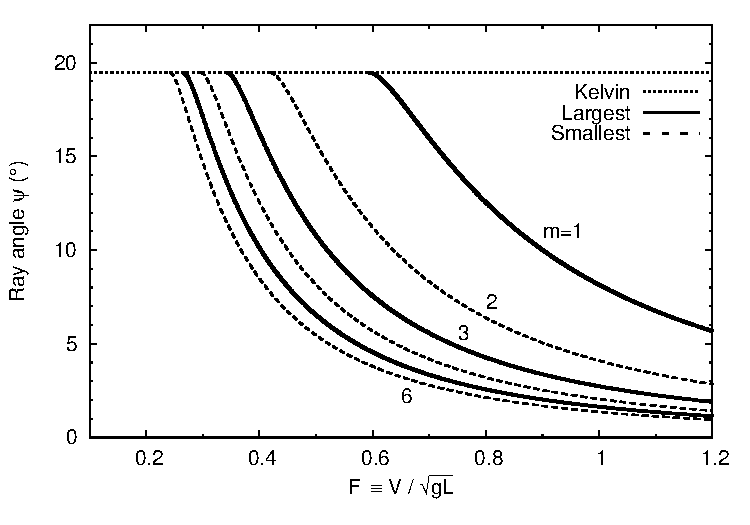
\includegraphics[height=0.33\textwidth]{chap6/xintrf}
    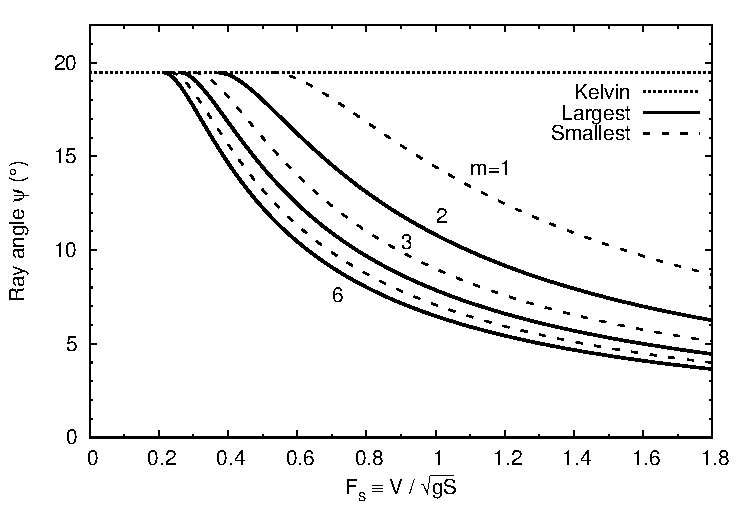
\includegraphics[height=0.33\textwidth]{chap6/yintrf}
  \bicaption[fig:psixym]{纵向干涉和横向干涉的主要差异}
  {左图是式\eqref{eq:psixm-a}给出的射线角$\psi_m^x$,其中$1\le m\le6$,
  $\ell=0.9$。右图是式\eqref{eq:psiym-a}给出的射线角$\psi_m^y$,其中$1\le m\le6$。
图中实线代表波幅极大,虚线代表波幅极小。}{Fig}
{Left side: ray angles $\psi^x_m$ given by \eqref{eq:psixm-a} with $\ell=0.9$ and
  $1\leq m\leq 6$. Right side: ray angles $\psi^y_m\hspace{0.05em},$ given by
 (\ref{eq:psiym-a}) with $1\leq m\leq 6$. Largest or smallest waves are 
 shown with solid or dashed lines.}
\end{figure}
%

现在解释图\ref{fig:psixym}左边和右边的重大区别。图\ref{fig:psixym}左边当$m=1$时
$\psi_1^x$对应纵向相长干涉,因而该处波幅极大。所以可以预期$\psi_1^x<|\psi|<\psi^K$
范围内的波浪波高小于沿射线$\psi=\pm\psi_1^x$的波浪的波高,因此单体船兴波角
的上界可以由$\psi_{\max}\approx\psi_1^x$给出,正如\parencite{Noblesse2014Why}
所述。然而图\ref{fig:psixym}右边当$m=1$时$\psi_1^y$对应横向相消干涉,因而该处
波幅极小。所以可以预期$\psi_1^y<|\psi|<\psi^K$范围内的波浪的波高大于沿射线
$\psi=\pm\psi_1^y$的波浪的波高。实际上,在Kelvin臂$\psi^K$的波浪的波高可能
会大于$\psi=\pm\psi_2^y$的波浪的波高。因此,双体船的波浪干涉效应可能会在
$\psi_1^y<|\psi|<\psi^K$的扇形区域内产生波高最大的波浪(将由进一步的数值
计算展示)。因此,$\psi_2^y$不一定是双体船兴波角的上限,波高最大的波浪也可能
出现在$\psi_1^y<|\psi|\le\psi^K$范围内。

\section{数值示例}
\label{sec:numillustrat}

可能在发生在双体船的情况的一个数值示例在图\ref{fig:ampl}中展示。
图\ref{fig:ampl}的顶部或底部分别展示了一艘片体间距为$s=0.2$或$s=0.5$的双体船
在$F_s=1$,1.7,2.5和3四个Froude数情况下产生的散波的波幅。双体船的船体形状
由式\eqref{eq:cathull}定义,并且$n=2$,$b=0.075$,$d=0.05$,即表\ref{tab:7cathull}
中名为Medium的船体。
%
\begin{figure}
\centering
\subfigure[$s=0.2$]
{
\label{fig:ampl-a}
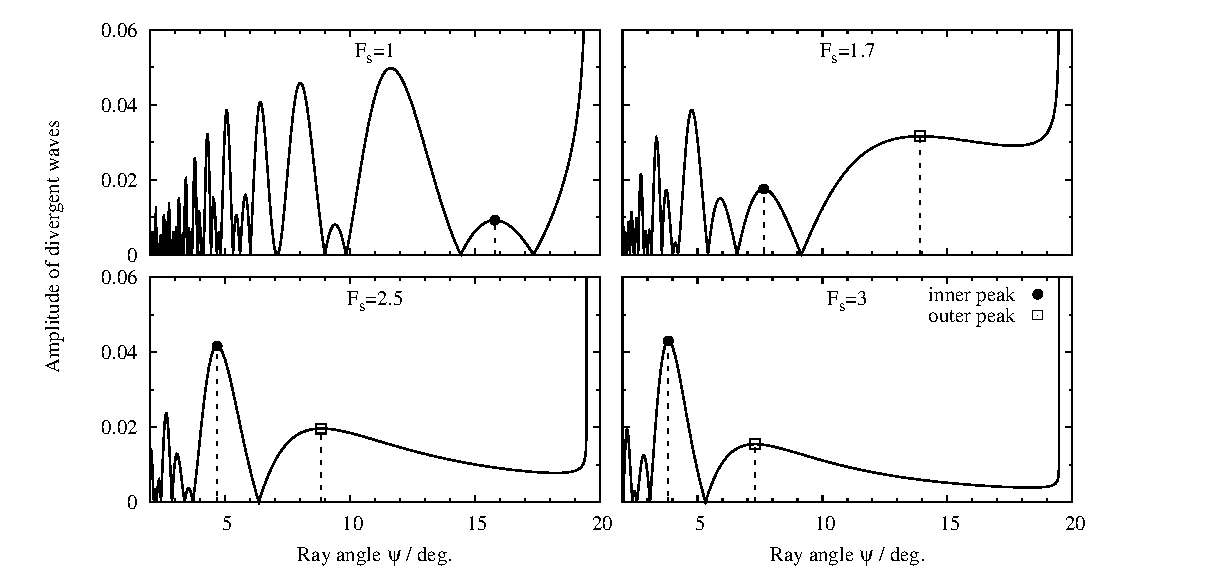
\includegraphics[width=16cm]{chap6/ampf-s2.pdf}
}\\
\subfigure[$s=0.5$]
{
\label{fig:ampl-b}
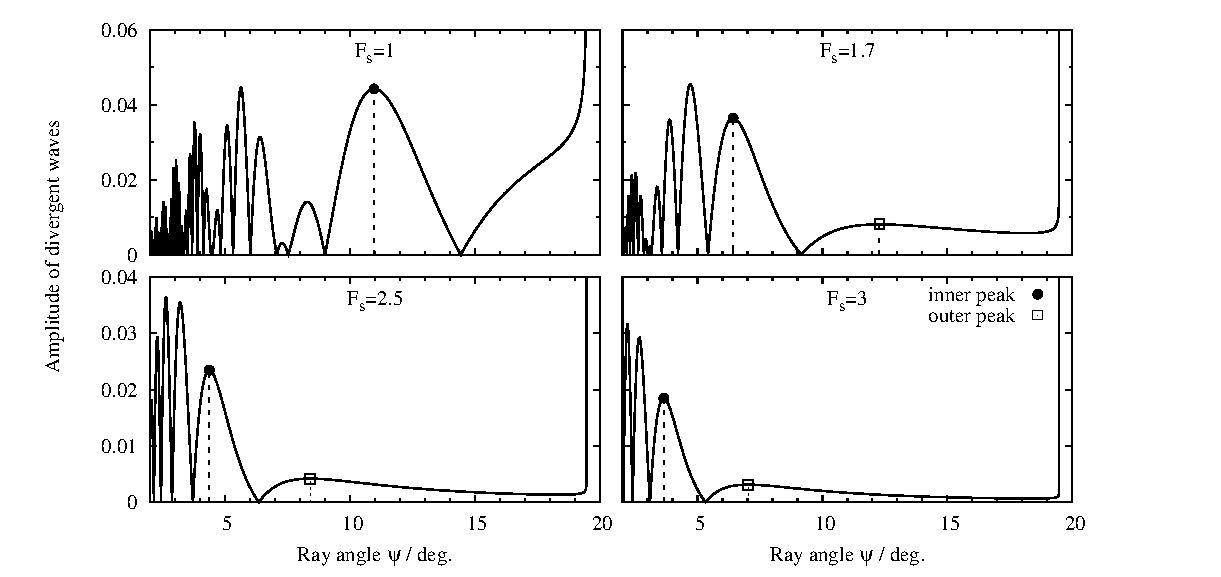
\includegraphics[width=16cm]{chap6/ampf-s5.pdf}
}
 \bicaption[fig:ampl]
 {双体船散波的波幅}
 {一艘片体间距为$s=0.2$(顶部)或$s=0.5$(底部)的双体船在$F_s=1$,1.7,2.5和3
 四个Froude数情况下产生的散波的波幅。外峰和第一个内峰分别虚线和开口的方形
 或实心圆表示}{Fig}
 {Amplitude of the divergent waves created by a catamaran with hull spacing $s=0.2$ (top) or $s=0.5$ 
 (bottom) for $2^\circ\!\leq\psi<19^\circ28'$ and four Froude numbers $F_s=1,$ 1.7, 2.5 and 3\hspace{0.05em}.  The outer 
 peak and the first inner peak are marked by dashed vertical lines with an open square or a solid circle, respectively.}
\end{figure}
%

图\ref{fig:ampl}中展示的和此后计算的散波的波幅由第\ref{chap:monohull}章所述
的方法所述。具体来说,波幅是用Hogner近似和驻相法计算的远场波的Fourier-Kochin表达式
中的波幅函数。图\ref{fig:ampl}中波幅在$\psi\approx19^\circ28'$是无界的,
因为驻相近似法在Kelvin臂$\psi=\pm\psi^K$是弱奇性的,因此在Kelvin臂及其附近是无效的。
特别地,传统的驻相近似法预测散波的波幅$a$在$\psi\approx\pm\psi^K$附近形如
$a\propto(\psi\mp\psi^K)^{-1/4}$。图\ref{fig:ampl}表明受奇性影响的范围在
$F_s=3$和$F_s=2.5$时是非常小的,但是随着$F_s$的减小而增大。这一范围在$F_s=1.7$
和$F_s=1$时可能较为明显。此外,在$\psi=\pm\psi^K$除了需要考虑散波还需考虑横波。
因此,图\ref{fig:ampl}和此后计算的波幅在Kelvin臂附近是无效的,正如
第\ref{chap:monohull}章所述。

图\ref{fig:ampl}中用竖线和实心圆表示的峰对应于图\ref{fig:psixym}
右侧第一个横向相长干涉$m=2$对应的射线角$\psi_2^y$,并且实际上可以用式
\eqref{eq:psiymapprox}近似。此峰今后称为``内峰'',并用$\psi=\pm\psi^i$表示。
内峰在图\ref{fig:ampl}的八种情况下都可以观察到。图中另一个用竖线和开口方形
表示,只在六种情况下可以观察到,即$s=0.2$和$s=0.5$和$F_s=1.7$,2.5和3。
此峰今后称为``外峰'',并用$\psi=\pm\psi^o$表示。外峰位于$\psi^i<\psi^o<\psi^K$
范围内。在$F_s=1$时,图\ref{fig:ampl}上半部分($s=0.2$)和下半部分($s=0.5$)的左上
四分之一不能观察到外峰。

图\ref{fig:ampl}的下半部分表明在大的片体间距$s=0.5$时(对应宽的双体船),内峰高于外
峰,并且比外峰更锐利。图\ref{fig:ampl}的下半部分表明在相对较小的片体间距$s=0.2$
(对应窄的双体船),在高Froude数$F_s=3$和$F_s=2.5$时内峰比外峰高且锐利。
但是在$s=0.2$且$F_s=1.7$的情况下(对应窄且慢的双体船),外峰可以高于内峰。

因此,图\ref{fig:ampl}暗示在大片体间距$s$或高Froude数$F_s$时(对应宽或快的双体船),
内峰$\psi^i$要高于外峰$\psi^o$。然而,在小片体间距且低Froude数情况下
(对应窄且慢的双体船)外峰$\psi^o$高于内峰$\psi^i$。这个一般性结论将被进一步的
系统计算证实和量化。

图\ref{fig:ampl}还展示了一些紧密相间的窄峰,这些峰对应射线角$\psi<\psi^i$的
相长干涉。这些另外的内峰可以高于第一个内峰$\psi^i$。因此通过波幅最大的波浪所在
的射线得到主要兴波角$\psi=\pm\psi_{\max}$的方法相对复杂,涉及某种程度的不确定性
和任意性,尤其是因为$|\psi|<\psi^i$的峰值是紧密相间的窄峰。
特别地,是这些窄峰在船波的观测中更突出,还是较宽的内峰$\psi^i$或外峰$\psi^o$
更容易被观察到,不是显而易见的。然而不管在何种情况下,外峰$\psi^o$或内峰$\psi^i$
都提供了主要兴波角$\psi=\pm\psi_{\max}$的上界,此后的计算只确定外峰和内峰。



\section{内峰}
\label{sec:inner}
图\ref{fig:psii}展示了数值确定的由表\ref{tab:7cathull}定义的七个片体在六个片体
间距$s=0.2$,0.3,0.4,0.5,0.6和0.8情况下共42个双体船在Froude数
$0.4<F_s\le3.5$范围内散波波幅的内峰。图中还展示了Kelvin角$\psi^K$和式
\eqref{eq:psiymapprox}给出的通过两点兴波模型预测的解析式$\psi^y_{\max}$。
图\ref{fig:psii}中以曲线$\psi=\pm\psi^y_{\max}$为中心的灰色窄带对应于
$\psi^y_{\max}-0.5^\circ\le\psi\le\psi^y_{\max}+0.5^\circ$。
%
\begin{figure}[htp]
  \centering
  \captionstyle{\centering}
    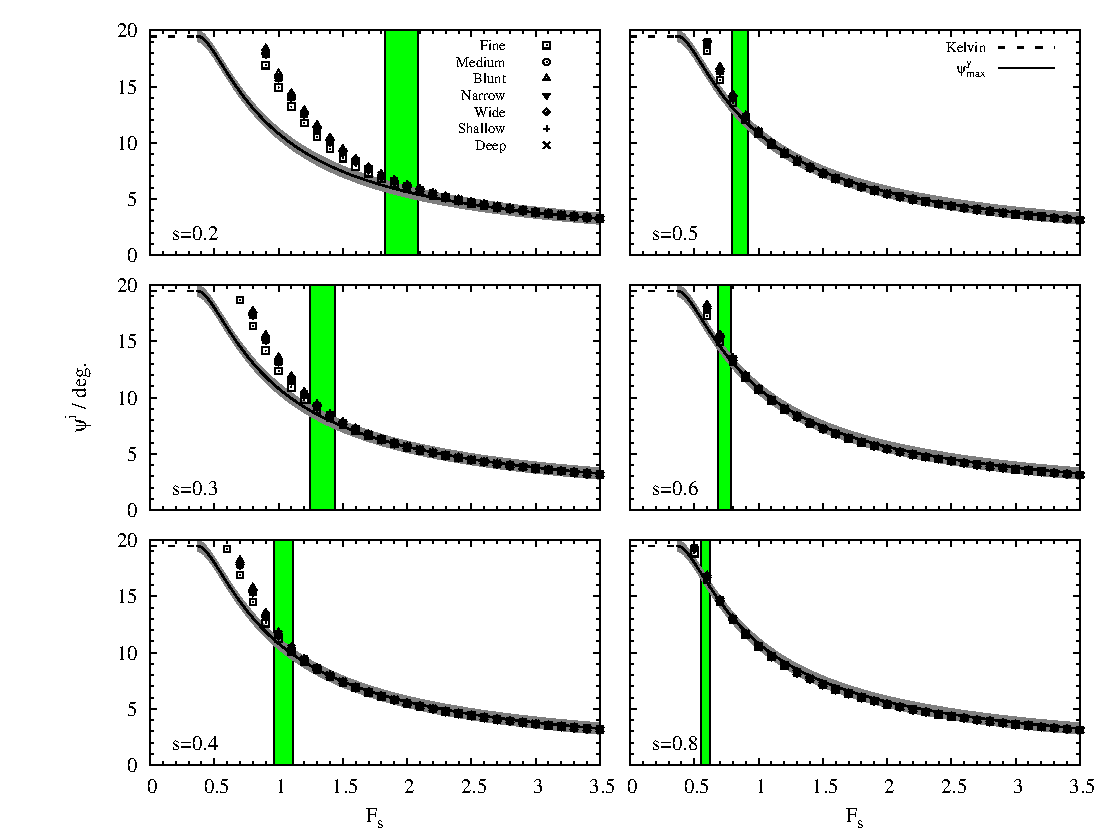
\includegraphics[width=14cm]{chap6/inner.pdf}
    \bicaption[fig:psii]{双体船散波波幅的内峰}{数值确定的由表\ref{tab:7cathull}
  定义的七个片体在六个片体间距$0.2\le s \le 0.8$情况下共42个双体船在
  Froude数$0.4<F_s\le 3.5$范围内
散波波幅的内峰}{Fig}{Numerically-determined ray angles $\psi^i$ associated with the 
  first inner peaks of the amplitudes of the 
  divergent waves created by 42 catamarans that correspond to the six hull spacings
  $s=0.2,$ 0.3, 0.4, 0.5, 0.6, 0.8 and the seven demi-hulls defined in 
  Table \ref{tab:7cathull} at Froude numbers $F_s$ within the range 
  $0.4<F_s \le 3.5\hspace{0.05em}.$ }
\end{figure}

图\ref{fig:psii}显示由式\eqref{eq:cathull}和表\ref{tab:7cathull}定义七艘船体的
内峰$\psi=\psi^i$的差异不大。因此,内峰受船体形状的影响很弱。此外,图\ref{fig:psii}
还表明数值确定的$\psi^i$与式\eqref{eq:psiymapprox}给出的解析式接近。
在大片体间距$s$或大Froude数时,即对于宽或快的双体船,计算得到的射线角
$\psi^i$与解析近似$\psi^y_{\max}$特别接近。但是在$s$和$F_s$较小时,即
对于窄且慢的双体船,计算得到的$\psi^i$明显大于近似$\psi^y_{\max}$。

计算得到的$\psi^i$和简单解析近似$\psi^y_{\max}$之间的差距在图\ref{fig:psii}中
用绿色竖直条带来量化。这些竖直条带展示了由式$\psi^i=\psi^y_{\max}+0.5^\circ$
决定的Froude数$F_s^i$。因此,当$F>F_s^i$时,计算得到的$\psi^i$超出$\psi^y_{\max}$
不到$0.5^\circ$。绿色条带的宽度展示了七艘船的分界Froude数$F_s^i$的差异。
图\ref{fig:psii}表明当$s$较小时,条带宽度较大,且对应较大的Froude数。
这个数值结果进一步阐明了对于宽或快的双体船,计算得到的$\psi^i$与近似式
$\psi^y_{\max}$很接近的结论。


图\ref{fig:bdry}展示了与25个片体间距$0.2\le s\le 0.8$和表\ref{tab:7cathull}定义
的七个片体间距对应的175个双体船的分界Froude数$F^i_s$(顶部)和关联的$sF_s^i$
(顶部)。图\ref{fig:bdry}中的绿色条带标示了计算中考虑的七个片体的$sF_s^i$
或$F_s^i$的变化。图\ref{fig:bdry}的顶部表明简单线性近似$sF_s^i\approx0.39+0.13s$
与绿色条带的上边界吻合较好。因此,决定$\psi^i-\psi^y_{\max}\le0.5^\circ$
的分界Froude数$F_s^i$的上界可以近似为
\begin{equation}
  F_s^i\approx0.13+0.39/s
  \label{eq:Fsi}
\end{equation}
图\ref{fig:bdry}还展示了替代的Froude数$F_s^i$
\begin{equation}
  F_s^i\approx0.13+0.47/s
  \label{eq:Fsisubs}
\end{equation}
图\ref{fig:psii}和图\ref{fig:bdry}表明当$F_s>F_s^i$时,其中$F_s^i$由\eqref{eq:Fsi}
或更严格的边界\eqref{eq:Fsisubs}给出,
第一个内峰$\psi^i$可以用$\psi^y_{\max}$很好地近似。今后将使用更加严格的
边界\eqref{eq:Fsisubs}代替\eqref{eq:Fsi},因为它可以为进一步考虑的内峰$\psi^i$
的估计提高稍微准确些的近似。
\begin{figure}[htp]
  \centering
  \captionstyle{\centering}
    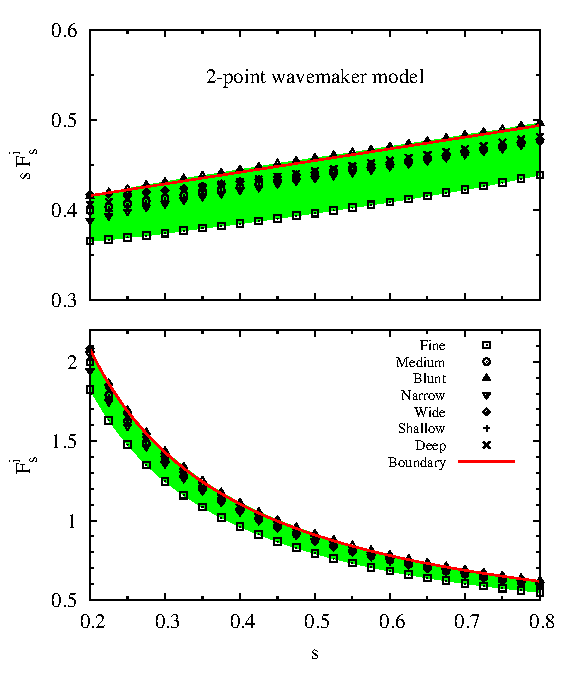
\includegraphics[width=14cm]{chap6/Fsi.pdf}
    \bicaption[fig:bdry]{分界Froude数$F_s^i$}
    {与25个片体间距$0.2\le s\le 0.8$和表\ref{tab:7cathull}定义的七个片体
  对应的175个双体船的分界Froude数$F_s^i$(底部)和关联的$sF_s^i$(顶部)}
  {Fig}{Froude number $F^i_s$ (bottom) and related scaled Froude number $sF^i_s$ 
    (top) for 175 catamarans that correspond to 25 hull-separation distances $s$
    within the range $0.2 \le s \le 0.8$ and the seven demi-hulls defined 
    in Table \ref{tab:7cathull}.}
\end{figure}



\section{本章小结}
本章考虑在无限深广的静水中以航速$V$直线航行的双体船的窄V字形尾迹,
双体船由长$L$间距$S$的完全相同的片体组成。
船体周围的流场以分布在船体表面的点源产生的流场表示,而不是简化为位于
片体首部区域的两点的兴波。
本章对船体形状参数(长宽比、吃水船长比、宽度吃水比、水线进流角)在广泛范围内变化的
七艘简单船体在范围$0.4\le F_s\le 3.5$内的125个Froude数$F_s\equiv V/\sqrt{S}$
和在范围$0.2\le s \le 0.8$内的25个片体间距$s\equiv S/L$情况下进行了系统的
数值计算,总共计算了21875个不同的算例。
双体船远场波系中波幅极大的波浪
所在的射线$\psi=\pm\psi^i$和$\psi=\pm\psi^o$---即主要兴波角$\psi^i$
和$\psi^o$---由一种实用的数值方法确定。该方法基于数值确定通过Hogner近似
和驻项法计算的Fourier-Kochin表达式的波幅函数的两大峰值。
数值计算表明,船体形状对主要兴波角$\psi^i$和$\psi^o$的影响很弱。
这一数值发现的现实意义是,一般双体船的主要兴波角$\psi^i$和$\psi^o$
可以通过关于Froude数$F_s$和片体间距$s$的简单的解析式近似。这些近似解析式
在本章通过参数化计算得到。计算结果还表明,当$s$或$F_s$足够大时---
即对于或`宽'或`快'的双体船---横向干涉效应占主导。此外,对于或宽或快的双体船
,本章的计算表明,将双体船兴波简化为片体首部两点兴波的两点兴波模型的预测
是符合实际的。然而当$s$或$F_s$都小时---即对于既`窄'且`慢'的双体船---
波浪干涉效应更加复杂。第\ref{chap:monohull}章对于单体船和本章对于双体船
主要兴波角的分析表明,尽管一艘船兴波的波幅受船体形状的强烈影响,
远场波系中波幅最大的波浪所在的角度受船体形状的影响很弱,因此主要兴波角
主要是船兴波的运动学特性。


